\PassOptionsToPackage{svgnames,dvipsnames,svgnames}{xcolor}

\documentclass[nonacm]{acmart}
\settopmatter{printfolios=true,printccs=false,printacmref=false}

%% Conference information
%% Supplied to authors by publisher for camera-ready submission;
%% use defaults for review submission.
%% ?

%% Copyright information
%% Supplied to authors (based on authors' rights management selection;
%% see authors.acm.org) by publisher for camera-ready submission;
%% use 'none' for review submission.
\setcopyright{none}
%\setcopyright{acmcopyright}
%\setcopyright{acmlicensed}
%\setcopyright{rightsretained}
%\copyrightyear{2019}           %% If different from \acmYear

%% Bibliography style
\bibliographystyle{ACM-Reference-Format}
%% Citation style
%\citestyle{acmauthoryear}  %% For author/year citations
%\citestyle{acmnumeric}     %% For numeric citations
%\setcitestyle{nosort}      %% With 'acmnumeric', to disable automatic
                            %% sorting of references within a single citation;
                            %% e.g., \cite{Smith99,Carpenter05,Baker12}
                            %% rendered as [14,5,2] rather than [2,5,14].
%\setcitesyle{nocompress}   %% With 'acmnumeric', to disable automatic
                            %% compression of sequential references within a
                            %% single citation;
                            %% e.g., \cite{Baker12,Baker14,Baker16}
                            %% rendered as [2,3,4] rather than [2-4].


%% Some recommended packages.
\usepackage{booktabs}   %% For formal tables:
                        %% http://ctan.org/pkg/booktabs
\usepackage{subcaption} %% For complex figures with subfigures/subcaptions
                        %% http://ctan.org/pkg/subcaption

\usepackage{microtype}
\usepackage{mdframed}
\usepackage{colortab}
\usepackage{mathpartir}
\usepackage{enumitem}
\usepackage{bbm}
\usepackage{stmaryrd}
\usepackage{mathtools}
\usepackage{leftidx}
\usepackage{todonotes}
\usepackage{xspace}
\usepackage{wrapfig}
\usepackage{float}

\usepackage{listings}%
\lstloadlanguages{ML}
\lstset{tabsize=2, 
basicstyle=\footnotesize\ttfamily, 
% keywordstyle=\sffamily,
commentstyle=\itshape\ttfamily\color{gray}, 
stringstyle=\ttfamily\color{purple},
mathescape=false,escapechar=\#,
numbers=left, numberstyle=\scriptsize\color{gray}\ttfamily, language=ML, showspaces=false,showstringspaces=false,xleftmargin=10pt, 
morekeywords={string, float, int},
classoffset=0,belowskip=\smallskipamount, aboveskip=\smallskipamount,
moredelim=**[is][\color{red}]{SSTR}{ESTR}
}
\newcommand{\li}[1]{\lstinline[basicstyle=\ttfamily\fontsize{9pt}{1em}\selectfont]{#1}}
\newcommand{\lismall}[1]{\lstinline[basicstyle=\ttfamily\fontsize{9pt}{1em}\selectfont]{#1}}
\newcommand{\dd}{\emph{delta dict}}
\newcommand{\mapP}{\{0 \rightarrow \text{"a"}, 1 \rightarrow \text{"b"}, 3 \rightarrow \text{"c"}, 6 \rightarrow \text{"d"}, 10 \rightarrow \text{"e"}\}}

%% Joshua Dunfield macros
\def\OPTIONConf{1}%
\usepackage{joshuadunfield}

%% Can remove this eventually
\usepackage{blindtext}

\usepackage{enumitem}

% \newtheorem{theorem}{Theorem}[chapter]
% \newtheorem{lemma}[theorem]{Lemma}
% \newtheorem{corollary}[theorem]{Corollary}
% \newtheorem{definition}[theorem]{Definition}
% \newtheorem{assumption}[theorem]{Assumption}
% \newtheorem{condition}[theorem]{Condition}

\newtheoremstyle{slplain}% name
  {.15\baselineskip\@plus.1\baselineskip\@minus.1\baselineskip}% Space above
  {.15\baselineskip\@plus.1\baselineskip\@minus.1\baselineskip}% Space below
  {\slshape}% Body font
  {\parindent}%Indent amount (empty = no indent, \parindent = para indent)
  {\bfseries}%  Thm head font
  {.}%       Punctuation after thm head
  { }%      Space after thm head: " " = normal interword space;
        %       \newline = linebreak
  {}%       Thm head spec
\theoremstyle{slplain}
\newtheorem{thm}{Theorem}  % Numbered with the equation counter
\numberwithin{thm}{section}
\newtheorem{defn}[thm]{Definition}
\newtheorem{lem}[thm]{Lemma}
\newtheorem{prop}[thm]{Proposition}
% \newtheorem{cor}[section]{Corollary}     
% \newtheorem{lem}[section]{Lemma}         
% \newtheorem{prop}[section]{Proposition}  

% \setlength{\abovedisplayskip}{0pt}
% \setlength{\belowdisplayskip}{0pt}
% \setlength{\abovedisplayshortskip}{0pt}
% \setlength{\belowdisplayshortskip}{0pt}

\fancyfoot{} % suppresses the footer (also need \thispagestyle{empty} after \maketitle below)

% !TEX root = main.tex

\newcommand{\mynote}[3]{\textcolor{#3}{\textsf{{#2}}}}
\newcommand{\rkc}[1]{\mynote{rkc}{#1}{blue}}
\newcommand{\nick}[1]{\mynote{cy}{#1}{purple}}

\newcommand{\cvert}{{\,{\vert}\,}}

%% https://tex.stackexchange.com/questions/9796/how-to-add-todo-notes
\newcommand{\rkcTodo}[1]{\todo[linecolor=blue,backgroundcolor=blue!25,bordercolor=blue]{#1}}

\newcommand{\mattTodo}[1]{\todo[linecolor=green,backgroundcolor=green!2,bordercolor=green]{\tiny\textit{#1}}}
\newcommand{\mattOmit}[1]{\colorbox{yellow}{(Matt omitted stuff here)}}

\def\parahead#1{\paragraph{\textbf{#1.}}}
%% \def\paraheadNoDot#1{\paragraph{{\textbf{#1}}}}
\def\subparahead#1{\paragraph{\textit{#1.}}}
%% \def\paraheadindent#1{\paragraph{}\textit{#1.}}
%% \def\paraheadindentnodot#1{\paragraph{}\textit{#1}}

\newcommand{\ie}{i.e.}
\newcommand{\eg}{e.g.}
% \newcommand{\etc}{{\emph{etc.}}}
% \newcommand{\cf}{{\emph{cf.}}}
% \newcommand{\etal}{{\emph{et al.}}}

%% \newcommand{\hazel}{\ensuremath{\textsc{Hazel}}}
%% \newcommand{\sns}{\ensuremath{\textsc{Sketch-n-Sketch}}}
%% \newcommand{\deuce}{\ensuremath{\textsc{Deuce}}}
\newcommand{\Elm}{\ensuremath{\textsf{Elm}}}
\newcommand{\sns}{\ensuremath{\textrm{Sketch-n-Sketch}}}
\newcommand{\deuce}{\ensuremath{\textrm{Deuce}}}

\newcommand{\sectionDescription}[1]{\section{#1}}
\newcommand{\subsectionDescription}[1]{\subsection{#1}}
\newcommand{\subsubsectionDescription}[1]{\subsubsection{#1}}
%% \newcommand{\subsectionDescription}[1]{\subsection*{#1}}
\newcommand{\suppMaterials}{the Supplementary Materials}

\newcommand{\defeq}{\overset{\textrm{def}}{=}}

\newcommand{\eap}{action suggestion panel\xspace}
\newcommand{\Eap}{Action suggestion panel\xspace}

\newcommand{\myfootnote}[1]{\footnote{ #1}}

\def\sectionautorefname{Section}
\def\subsectionautorefname{Section}
\def\subsubsectionautorefname{Section}

\newcommand{\code}[1]{\lstinline{#1}}
\newcommand{\str}[1]
  {``#1''}

% Make italic?
%\newcommand{\Property}[1]{\emph{#1}}
\newcommand{\Property}[1]{\textrm{#1}}

% Calling out Cyrus's favorite verb, 'to be' ;)
\newcommand{\IS}{\colorbox{red}{is}\xspace}

\newcommand{\codeSize}
  %% {\footnotesize}
  {\small}

%\newcommand{\JoinTypes}[2]{\textsf{join}~~#1~~#2}
\newcommand{\JoinTypes}[2]{\textsf{join}(#1,#2)}

%% \newtheorem{theorem}{Theorem}[section] % 2.1, 2.2, etc.
\newtheorem{theorem}{Theorem}             % 1, 2, etc.
\newtheorem{remark}[theorem]{Remark}

%%%%%%%%%%%%%%%%%%%%%%%%%%%%%%%%%%%%%%%%%%%%%%%%%%%%%%%%%%%%%%%%%%%%%%%%%%%%%%%%
%% Spacing

\newcommand{\sep}{\hspace{0.06in}}
\newcommand{\sepPremise}{\hspace{0.20in}}
\newcommand{\hsepRule}{\hspace{0.20in}}
\newcommand{\vsepRuleHeight}{0.08in}
\newcommand{\vsepRule}{\vspace{\vsepRuleHeight}}
\newcommand{\miniSepOne}{\hspace{0.01in}}
\newcommand{\miniSepTwo}{\hspace{0.02in}}
\newcommand{\miniSepThree}{\hspace{0.03in}}
\newcommand{\miniSepFour}{\hspace{0.04in}}
\newcommand{\miniSepFive}{\hspace{0.05in}}
\newcommand{\breakAndIndent}
  {\mbox{}

   %% \hspace{0.15in}
   \hspace{0.00in}
  }

\newcommand{\justIndent}
  %% {\hspace{0.15in}
  {\hspace{0.00in}
  }

%%%%%%%%%%%%%%%%%%%%%%%%%%%%%%%%%%%%%%%%%%%%%%%%%%%%%%%%%%%%%%%%%%%%%%%%%%%%%%%%

% \lstset{
% %mathescape=true,basicstyle=\fontsize{8}{9}\ttfamily,
% literate={=>}{$\Rightarrow$}2
%          {<=}{$\leq$}2
%          {->}{${\rightarrow}$}1
%          {\\\\=}{\color{red}{$\lambda$}}2
%          {\\\\}{$\lambda$}2
%          {**}{$\times$}2
%          {*.}{${\color{blue}{\texttt{*.}}}$}2
%          {+.}{${\color{blue}{\texttt{+.}}}$}2
%          {<}{${\color{green}{\lhd}}$}1
%          {>?}{${\color{green}{\rhd}}$?}2
%          {<<}{${\color{green}{\blacktriangleleft}}$}1
%          {>>?}{${\color{green}{\blacktriangleright}}$?}2
%          {\{}{${\color{blue}{\{}}$}1
%          {\}}{${\color{blue}{\}}}$}1
%          {[}{${\color{purple}{[}}$}1
%          {]}{${\color{purple}{]}}$}1
%          {(}{${\color{darkgray}{\texttt{(}}}$}1
%          {)}{${\color{darkgray}{\texttt{)}}}$}1
%          {]]}{${\color{gray}{\big(}}$}1
%          {]]}{${\color{gray}{\big)}}$}1
% }

%%%%%%%%%%%%%%%%%%%%%%%%%%%%%%%%%%%%%%%%%%%%%%%%%%%%%%%%%%%%%%%%%%%%%%%%%%%%%%%%

\newcommand{\li}[1]{\lstinline[basicstyle=\ttfamily\fontsize{9pt}{1em}\selectfont]{#1}}
\newcommand{\lismall}[1]{\lstinline[basicstyle=\ttfamily\fontsize{9pt}{1em}\selectfont]{#1}}
\newcommand{\mapP}{\{0 \rightarrow \text{"a"}, 1 \rightarrow \text{"b"}, 3 \rightarrow \text{"c"}, 6 \rightarrow \text{"d"}, 10 \rightarrow \text{"e"}\}}
\newcommand{\dictP}{[(0, "a"), (0, "b"), (1, "c"), (2, "d"), (3, "e")]}

%%%%%%%%%%%%%%%%%%%%%%%%%%%%%%%%%%%%%%%%%%%%%%%%%%%%%%%%%%%%%%%%%%%%%%%%%%%%%%%%

%% \newcommand{\sal}{simple association list}
\newcommand{\sal}{association list}
\newcommand{\Sal}{Association List}

%% \newcommand{\cal}{canonicalized association list}
\newcommand{\cal}{canonical association list}
\newcommand{\Cal}{Canonical Association List}
\newcommand{\Cals}{Canonical association lists}

%% \newcommand{\fpf}{finite partial function}
\newcommand{\fpf}{partial function}
\newcommand{\Fpf}{Partial Function}
\newcommand{\Fpfs}{Partial functions}

\newcommand{\dd}{delta dictionary}
\newcommand{\dds}{delta dictionaries}
\newcommand{\Dd}{Delta Dictionary}
\newcommand{\Ddls}{Delta dictionaries}

%%%%%%%%%%%%%%%%%%%%%%%%%%%%%%%%%%%%%%%%%%%%%%%%%%%%%%%%%%%%%%%%%%%%%%%%%%%%%%%%

\newcommand{\SemTot}{Semantic Totality}
%% \newcommand{\SemInj}{Semantic Injectivity}
\newcommand{\SemInj}{Extensionality}
\newcommand{\EqDec}{Decidable Equality}
%% \newcommand{\EzDstr}{Ease of Destruction}
\newcommand{\EzDstr}{Easy Destructibility}

%% tweak and remove indirection macros later, once terminology settles
\newcommand{\Total}{\SemTot}
\newcommand{\Extensional}{\SemInj}
\newcommand{\DecidableEq}{\EqDec}
\newcommand{\Destructible}{\EzDstr}

\newcommand{\total}{Total}
\newcommand{\extensional}{Extensional}
\newcommand{\decidable}{Decid. Eq.}
\newcommand{\destructible}{Destructible}

\newcommand{\semanticallyTotal}{Semantically Total}
\newcommand{\destructed}{Destructed}

%%%%%%%%%%%%%%%%%%%%%%%%%%%%%%%%%%%%%%%%%%%%%%%%%%%%%%%%%%%%%%%%%%%%%%%%%%%%%%%%

% for use in alltt
\newcommand{\altFAll}{\ensuremath{\forall}}
\newcommand{\altRArr}{\ensuremath{\rightarrow}}
\newcommand{\altRARR}{\ensuremath{\Rightarrow}}
\newcommand{\altVdash}{\ensuremath{\vdash}}
\newcommand{\altTimes}{\ensuremath{\times}}
\newcommand{\altAnd}{\ensuremath{\land}}
\newcommand{\altOr}{\ensuremath{\lor}}
\newcommand{\altNE}{\ensuremath{\ne}}
\newcommand{\altEmpty}{\ensuremath{\varnothing}}
\newcommand{\altIn}{\ensuremath{\in}}
\newcommand{\altNIn}{\ensuremath{\notin}}
\newcommand{\altSum}{\ensuremath{\sum}}
\newcommand{\altLAng}{\ensuremath{\langle}}
\newcommand{\altRAng}{\ensuremath{\rangle}}
\newcommand{\altLamb}{\ensuremath{\lambda}}
\newcommand{\altGam}{\ensuremath{\Gamma}}
\newcommand{\altCirc}{\ensuremath{\circ}}
\newcommand{\altCdot}{\ensuremath{\cdot}}
\newcommand{\altBot}{\ensuremath{\bot}}

\input{macros}

%\setlength{\abovecaptionskip}{4pt plus 3pt minus 2pt} % Chosen fairly arbitrarily
%\setlength{\belowcaptionskip}{-4pt plus 3pt minus 2pt} % Chosen fairly arbitrarily


\begin{document}

%% Title information
\title{A Deduped Dictionary Data Structure for Dependent Domains}

%% Author information
%% Contents and number of authors suppressed with 'anonymous'.
%% Each author should be introduced by \author, followed by
%% \authornote (optional), \orcid (optional), \affiliation, and
%% \email.
%% An author may have multiple affiliations and/or emails; repeat the
%% appropriate command.
%% Many elements are not rendered, but should be provided for metadata
%% extraction tools.

% ACM member number: ?
% \author{?}
% \authornote{with author1 note}          %% \authornote is optional;
                                        %% can be repeated if necessary
% \orcid{nnnn-nnnn-nnnn-nnnn}             %% \orcid is optional
%\affiliation{
%  \position{Graduate student}
%  % \department{Department1}              %% \department is recommended
%  \institution{University of Chicago}            %% \institution is required
%  % \streetaddress{Street1 Address1}
%  % \city{City1}
%  % \state{State1}
%  % \postcode{Post-Code1}
%  % \country{Country1}
%}
%\email{nickmc@uchicago.edu}          %% \email is recommended

%% Paper note
%% The \thanks command may be used to create a "paper note" ---
%% similar to a title note or an author note, but not explicitly
%% associated with a particular element.  It will appear immediately
%% above the permission/copyright statement.
% \thanks{with paper note}                %% \thanks is optional
                                        %% can be repeated if necesary
                                        %% contents suppressed with 'anonymous'

TODO TODO TODO remaining info, e.g. ACM member number and author info or whatev

%% Abstract
%% Note: \begin{abstract}...\end{abstract} environment must come
%% before \maketitle command
% !TEX root = ?.tex

%% no citations in Abstract
%%
%% \cite{?}

\begin{abstract}

Dictionaries, or finite maps, are a core data structure in any programming language.
%
General-purpose languages implement dictionaries with hash tables or balanced trees, but proof assistants---which favor simplicity and provability over performance---generally employ association lists or finite partial functions.
%
Though suitable for many uses, each solution has drawbacks:
%
association lists allow arbitrary order and may contain duplicates (unless refined with an explicit proof about validity), and
%
partial functions cannot be compared for equality
%
nor easily destructed.

We develop a novel list-based representation, called \emph{delta dictionaries}, that simultaneously achieves benefits of the conventional representations.
%
Delta dictionaries are \emph{total} (every type-correct list is semantically valid),
%
\emph{extensional} (there is a one-to-one correspondence between lists and semantic mappings), and
%
\emph{destructible} (the internal representation can be inspected as needed).
%
We present the implementation of delta dictionaries and relevant metatheory---formalized in Agda---and we discuss when delta dictionaries may or may not be preferable to conventional solutions.

%% Using a variant of delta-encoding, we develop a novel list-based solution that preserves
%% canonical ordering while ensuring that every type-correct list is semantically valid, eliminating the need for refinement
%% with a proof of validity. Our solution also establishes a one-to-one correspondence between dictionary terms and semantic
%% mappings. We demonstrate the practical importance of these properties when developing metatheory for environment-based
%% evaluation semantics, while acknowledging that drawbacks of our solution may make it inferior to one of the conventional
%% solutions in some cases where that conventional solution is viable. We prove the relevant metatheory in Agda.

%
% Our solution is not suitable for all key types, and is harder to destruct or
%iterate than other list-of-pair solutions, but is nonetheless better suited to many large, complex program
%foundations metatheories than the existing solutions.
%
% Although easy to define and reason about, this approach has the disadvantage that keys
%can be duplicated, leading to the fact that many distinct lists represent the same semantic mapping.
%This many-one relationship creates various difficulties when used in practice, such as when proving
%contraction and exchange for a type-checking judgment.

\end{abstract}

\input{defs}

%% Keywords
%% comma separated list
% \keywords{keyword1, keyword2, keyword3}  %% \keywords is optional
% \keywords{..., ...}

%% \maketitle
%% Note: \maketitle command must come after title commands, author
%% commands, abstract environment, Computing Classification System
%% environment and commands, and keywords command.
\maketitle
\thispagestyle{empty} % suppresses the footer

\section{Introduction}
Conventionally, the design of data structures and algorithms is chiefly focused on performance,
which is of significantly diminished concern in proof assistants. As such, proof assistants often
use entirely different data structures than those of conventional settings, with a focus on simplicity
or useful mathematical properties. Dictionaries - which serve a broad range of purposes but are
perhaps most familiar as implementations of type contexts and evaluation environments - are typically
implemented in one of the following manners: (TODO source for each)
\\\\
\newcommand{\lameq}[1]{$\lambda$ $x$ . $x == {#1}$}
\begin{tabular}{ l l }
 Naive list-of-pairs         & [(3, "c"), (1, "b"), {\color{gray} (3, "q")}, (6, "d")] \\
 Canonicalized list-of-pairs & [(1, "b"), (3, "c"), (6, "d")] \quad (insert function dedupes and preserves canonical order) \\
 Finite partial function     & \lameq{3} ? "c" : (\lameq{1} ? "b" : (\lameq{3} ? {\color{gray} "q"} : (\lameq{6} ? "d" : None) x) x) x
\end{tabular}
\\

The naive list-of-pairs solution is perhaps the most common, being trivially simple. Furthermore:
%\begin{itemize}
 (1) any list-of-pairs that type-checks represents a valid mapping,
       so there's no need to package the data with a proof term that asserts its validity,
 (2) it's trivial to destruct and iterate,
 (3) checking semantic equivalence of two dicts, while non-trivial, is decidable and not too difficult.
%\end{itemize}
 The major downside is that many distinct dicts
represent the same semantic mapping - because dicts are sensitive to duplication and ordering
of insertions, we cannot use equality primitives to check the semantic
equality of two dicts:
  \begin{figure}[H]
    \centering
    \begin{tikzpicture}[nodes = {align = left}]
      \node [scale=.45]
      {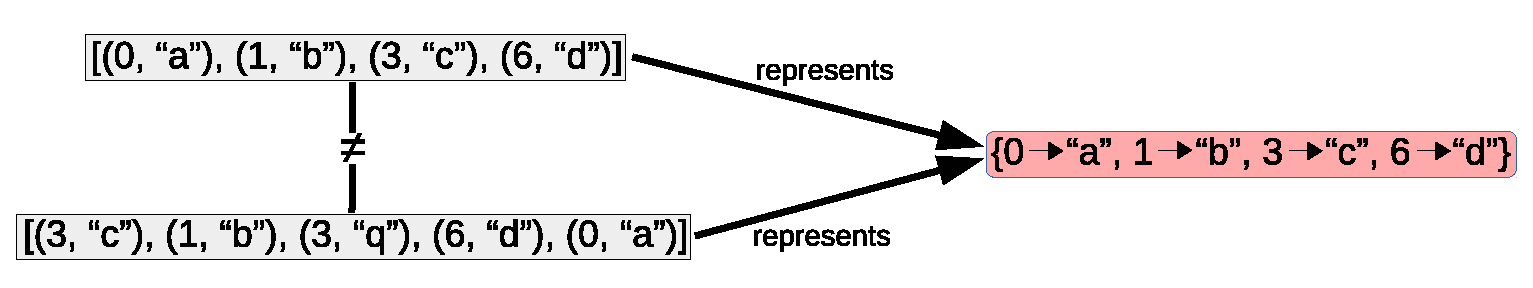
\includegraphics{figs/unequal.eps}};
    \end{tikzpicture}
    \caption{Same semantic mapping represented by unequal list-of-pair dicts}
    \label{fig:uneq}
  \end{figure}
This drawback is glaring when attempting to prove the \emph{structural properties} \emph{contraction}
and \emph{exchange} of a type checking judgment (or other judgments parameterized by some sort of context).
These properties correspond, respectively, to the irrelevance of duplication and reordering in a context
with regards to the judgment's conclusions. With the naive list-of-pairs solution, a separate proof must
be developed for each constructor in the language which actually uses the context (e.g. lets, lambdas,
case branches, etc.) to show that duplication or reordering in the context will not affect the results
of the judgment. Alternatively, if the data structure itself is insensitive to duplication and reordering
of insertions, then analogs of \emph{contraction} and \emph{exchange} can be proven for the data structure
itself. At this point the \emph{contraction} and \emph{exchange} of each judgment come "for free".
  %{\huge
  \begin{figure}[H]
    $
    \inferrule*[lab=\textbf{\large Contraction}]
      {\Gamma, (x, a), (x, b) \vdash T}
      {\Gamma, (x, b) \vdash T}
    $
    \quad\quad\quad\quad
    $
    \inferrule*[lab=\textbf{\large Exchange}]
      {\Gamma, (x, a), (y, b) \vdash T \\ x \ne y}
      {\Gamma, (y, b), (x, a) \vdash T}
    $
    \\\hfill\\\quad\quad
    $
      \Gamma, (x, a), (x, b) = \Gamma, (x, b)
    $
    \quad\quad
    $
      x \ne y \rightarrow \Gamma, (x, a), (y, b) = \Gamma, (y, b), (x, a)
    $
    \caption{Contraction and exchange theorems for type assignments $T$, as well as analogs for set-like data structures (TODO source for contraction and exchange)}
    \label{fig:con-exch}
  \end{figure}
  %}
Indeed, the other two conventional solutions (as well as ours) achieve the requisite set-like insensitivity
to duplication and reordering, yielding \emph{contraction} and \emph{exchange} "for free" and ensuring that
semantically equivalent dicts are also equal according to the built-in equality primitive\footnote{Finite partial
functions require the additional postulate of \emph{functional extensionality}, which can be postulated
at essentially no cost given that it's been proven consistent with the constructive calculi underlying most
popular proof assistants (TODO SOURCE)}. However, the other two conventional solutions have other drawbacks.
Canonicalized lists-of-pairs must retain a proof of validity to ensure that the dict is ordered and deduped.
Anytime the dict is "manipulated", a theorem must be invoked to generate a proof of validity for the new dict,
and this proof must be packaged with the new dict wherever it goes. This can be cumbersome, but an even bigger
problem occurs when the dict is used as data. For example, an evaluation rule may take an environment $E$ and
a lambda $\lambda x . e$ and produce a closure $[E] \lambda x . e$. Since $E$ must carry a proof term, it's no
longer possible to check equality of closures using equality primitives, and decidability of semantic equality
becomes problematic at best. With the finite partial function approach, equality is not decidable in the first
place, since the function type does nothing to guarantee that the function is actually finite.
Alternatively, the function could be packaged with a constructive proof that its support is finite, in which
case equality should be decidable, but then we run into the same problems we had before with proof terms and
proof relevance.

Our solution, which we dub {\dd}s, addresses the aforementioned problems by using a delta to
encode a key relative to its predecessor, instead of storing the key's literal value (details in section TODO(Mechanism)).
\\
\begin{tabular}{ l l }
 \quad\quad Delta dict & [(1, "b"), (1, "c"), (2, "d")]
\end{tabular}

Every list-of-pairs that type-checks is a valid \dd, and every unique \dd~ represents
a unique semantic mapping. So no proof term is needed to establish validity, there is a bijection between
\dd~ terms and finite maps, and the proof assistant's equality primitives, when applied to {\dd}s, correspond
exactly to semantic mapping equivalence. These properties make {\dd}s very suitable for use as contexts for
structural judgments or for use as data in the likes of closures.

Naturally, {\dd}s have some drawbacks as well. The use of deltas requires that the key type not merely be
ordered but also possess a difference operation and a least element. Our definition and implementation uses
natural numbers for keys, and in section TODO we illustrate how to use bijections to the naturals as a way
of supporting strings, integers, or other key types that can be bijected to the naturals without great
difficulty. Although most types that are suitable for use as keys in the first place can be bijected to the
naturals, for some types defining this bijection may be too awkward or cumbersome, in which case {\dd}s may
be a poor choice.

Another drawback is that destruction and iteration of {\dd}s is substantially more
difficult than it is with the conventional list-of-pair solutions, for which these operations are trivial
(finite partial functions cannot be properly destructed at all). Since the keys in a \dd~ are not represented
by their literal values, encapsulation disallows (TODO should disallow??) destruction (or other operations,
such as map) as though it were an ordinary list. Instead, destruction and deletion are offered only through
library functions, which guarantee that any \dd~ is either empty or that it can be destructed into a single
mapping and a \dd~ that when extended by that single mapping will equal the original \dd. Not only is it
more awkward to use a function for destruction than to use pattern matching, it also risks breaking
straightforward structural recursion, in some cases forcing the developer to establish termination manually.
The difficulties of destruction, and techniques for alleviating these difficulties, are discussed further in
section TODO. Analysis of the tradeoffs (in terms of lines-of-code required to prove metatheory) between more
difficult destruction vs more verbose proofs of \emph{contraction} and \emph{exchange}, is discussed in section
TODO(Evaluation), leading to soft recommendations about which solution best fits a particular scenario.

Finally, because they guarantee the \emph{structural properties} \emph{contraction} and
\emph{exchange}, {\dd}s are inherently inappropriate for substructural logics/judgments that reject one or
both of those properties. In these cases, the naive solution's sensitivity to duplication and/or ordering is
a feature, not a bug, and that solution becomes not only the natural solution but the morally correct one.
Future work could explore the possibility of data structures that uphold one of these properties but not the
other.

\begin{figure}[H]
  \begin{tabular}{ l | c | c | c | c | c | c}
                               & Simple & Always valid & Injective & Decidable equality & Destruction & Key type requirement
   \\\hline
   Naive list-of-pairs         & +1     & Yes          & No        & Yes                & Trivial     & Decidable equality
   \\\hline
   Canonicalized list-of-pairs & 0      & No           & Yes       & Yes                & Trivial     & Orderable
   \\\hline
   Finite partial function     & 0      & *            & Yes       & No                 & No          & Decidable equality
   \\\hline
   Delta dict                  & -1     & Yes          & Yes       & Yes                & Hard        & Bijects to naturals
  \end{tabular}
  \caption{The pros, cons, and other high-level properties of each solution}
  \label{fig:pros-cons}
\end{figure}

% something something "make impossible states impossible", and how this principle relates to refinements and
% proof terms in the domain of proof assistants

%ordering- and duplication-sensitive list-of-pairs: In particular,
%the \emph{structural properties} \emph{contraction} and \emph{exchange} of a type checking judgment (or
%other judgments parameterized by some sort of context) come almost "for free" if the context is represented by
%a set-like data structure that is agnostic to insertion order and which does not allow duplicate keys.
%This is a substantial benefit compared to deriving a separate proof of contraction and exchange for each
%judgment that takes a context parameter.

%alternative list-of-pairs approach that uses a variant of delta-encoding to maintain keys in sorted order
%while preventing duplication. As such, using one of these representations means \emph{contraction} and
%\emph{exchange} need be proven only once, for the dictionary itself, rather than a separate proof for each
%context-sensitive judgment. There are additional benefits of the ordering- and duplication-agnostic properties
%- the delta-encoding approach, in particular, has the additional property that physical equality is
%equivalent to semantic equivalence. However, they are not panaceas - the typical list-of-pair data structure
%is much easier to destruct and iterate than the new approaches, and the delta-encoding approach is limited
%to key types that are easily mapped to and from the natural numbers.

\section{Mechanism}
List-of-pairs with ordered, "delta-encoded" keys;
instead of storing the raw keys, we store
the difference from the previous key, minus 1
\begin{figure}[H]
  \centering
  \begin{tikzpicture}[nodes = {align = left}]
    \node [scale=.45]
    {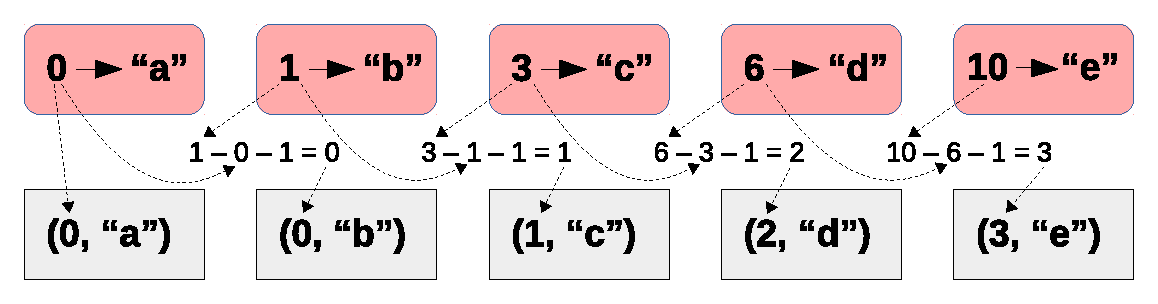
\includegraphics{figs/mech-1.eps}};
  \end{tikzpicture}
  \caption{How do we represent the mapping $\mapP$ as a \dd?}
  \label{fig:mech1}
\end{figure}
\begin{figure}[H]
  \centering
  \begin{tikzpicture}[nodes = {align = left}]
    \node [scale=.45]
    {\includegraphics{figs/find-6.eps}};
  \end{tikzpicture}
  \caption{How do we find key $6$ in the \dd?}
  \label{fig:find-6}
\end{figure}

TODO

\section{Metatheory}
TODO

\section{Evaluation}
TODO

\section{References}
TODO TODO TODO - REFERENCES
\\
the second answer on this stack overflow suggests the finite partial function approach:
\\
https://stackoverflow.com/questions/47362451/creating-a-dictionary-map-in-coq
\\
oh hey appears that this is in software foundations too
\\
https://6826.csail.mit.edu/2019/lf/Maps.html
\\
Coq has list-based maps that retain sorted order, but not every list data is a valid mapping
\\
https://coq.inria.fr/library/Coq.FSets.FMapList.html
\\
Coq also has FMapPositive, which is a tree based on the binary representation
\\
This one seems to attach a canonicity proof to an ordinary list:
\\
http://www.cs.bc.edu/~tassarot/papers/iris-refinement/coqdoc/iris.prelude.natmap.html

\clearpage
%\bibliography{references,all.short}
\bibliography{references}

% \clearpage
% \appendix
% \input{implementation-appendix}

\end{document}
